\section{Redegørelse af et ANN netværk}

\subsection{ANN's baggrund}
Et ANN(Artificial Neural Network) er en form for kunstig intellegens, hvor man prøver at efterligne den menneskelige hjerne
ved at lave simple versioner af det netværk af de mange milliarder neuroner der findes i den menneskelige hjerne.
Ligesom hvor en biologisk menneskehjerne har neuroner og synapser med forskellige styrker, så har et ANN også det, dog lidt simplere
så man kan tillægge værdier til de forskellige neuroner og synapser.

\subsection{Strukturen bag neuronerne i et ANN}
I den menneskellige hjerne er der som sagt milliarder af forskellige neuroner \footcite{DDOhjerne}.
I et ANN laver man ikke ligeså mange
neuroner som i en rigtig hjerne, da det er umuligt med den teknologi vi har i dag, men det er stadigvæk i fokus at lave et netværk med så mange neuroner
som muligt.
Derfor er det vigtigt at disse neuroner er matematisk set meget simple, så det er nemt for en moderne computer bare at blæse gennem matematikken
i et ANN. Dermen er den strukter man har valgt bag én neuron i et givet ANN vist i figur 1.

\begin{figure}
\label{neuron}
\caption{Model af en neuron}
\LARGE
\begin{center}
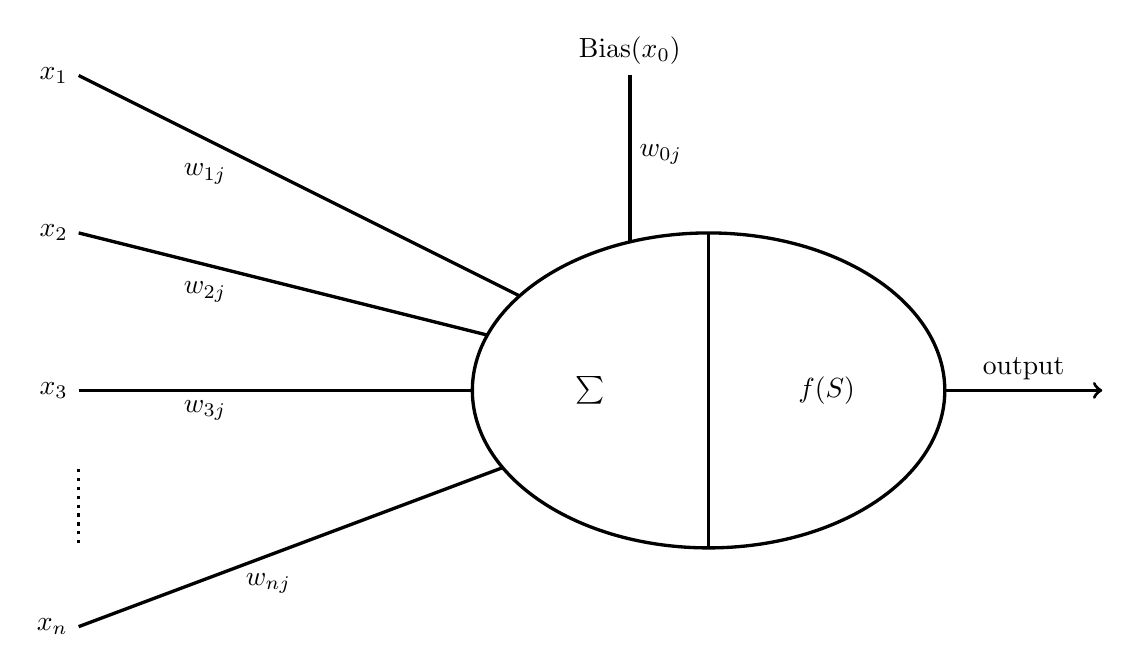
\begin{tikzpicture}

        \draw[very thick] (-1, 4) node[anchor=south]{Bias($x_0$)} -- (-1, 0);
        \draw[very thick] (-8, 4) node[anchor=east]{$x_1$} -- (0, 0);
        \draw[very thick] (-8, 2) node[anchor=east]{$x_2$} -- (0, 0);
        \draw[very thick] (-8, 0) node[anchor=east]{$x_3$} -- (0, 0);
        \draw[very thick, dotted] (-8, -1) -- (-8, -2);
        \draw[very thick] (-8, -3) node[anchor=east]{$x_n$}-- (0, 0);

        \node[anchor=west] at (-1, 3){$w_{0j}$};
        \node[anchor=north east] at (-6, 3){$w_{1j}$};
        \node[anchor=north east] at (-6, 1.5){$w_{2j}$};
        \node[anchor=north east] at (-6, 0){$w_{3j}$};
        \node[anchor=north west] at (-6, -2.2){$w_{nj}$};

        \draw[very thick, fill=white] (0, 0) ellipse (3 and 2);
        \draw[very thick] (0, 2) -- (0, -2);
        
        \node at (-1.5, 0){$\sum$};
        \node at (1.5, 0){$f(S)$};

        \draw[very thick, ->] (3, 0) -- (4, 0) node[anchor=south]{output} -- (5, 0);

\end{tikzpicture}
\end{center}
\normalsize

\end{figure}

Hvor alle $x_n$ er outputs fra andre neuroner der er tilsluttet denne neuron via synapser, $w_{nj}$ er såkaldte vægte der angiver hvor
forstærket signalet er fra outputtet af sidste neuron og bias er en værdi der der enten vil øge eller
sænke outputtet af en given neuron. Det der så sker inde i neuronen er to ting. \\
Først bliver alle inputs ganget sammen med deres vægte og summeret op. \\
Derefter bliver der ført en såkaldt "Activation function" der typisk bare normaliserer
summationen mellem f.eks 0 og 1\footcite{ANN11}. Her betragter jeg logistisk vækst med et maksimum på 1 som min activation function, hvor
funktionen vil så tage et vilkårligt tal og så spytte et andet tal ud der ligger mellem 0 og 1, jeg betegner funktionen med symbolet $sigma$\\
\includegraphics[width=\textwidth]{diagrammer/sigmoid.pdf}

Et ANN består af en hel masse neuroner fra figur 1 der er sammensat som på figur 2

\begin{figure}
\label{netvaerk}
\caption{Model af et neuralt netværk}
\LARGE
\begin{center}
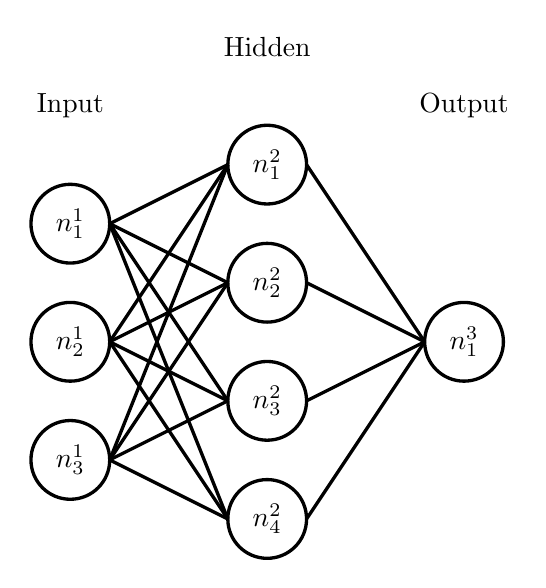
\begin{tikzpicture}

        \foreach \x in {1, 2, 3}
        {
                \draw[very thick] (0, -1.5*\x) circle (0.5);
                \node at (0, -1.5*\x) {$n_{\x}^1$};
                \foreach \y in {1, 2, 3, 4}
                {
                        \draw[very thick] (0.5, -1.5*\x) -- (2, -1.5*\y+0.75);
                }
        }

        \foreach \y in {1, 2, 3, 4}
        {
                \draw[very thick] (2.5, -1.5*\y+0.75) circle (0.5);
                \node at (2.5, -1.5*\y+0.75){$n_{\y}^2$};
                \draw[very thick] (3, -1.5*\y+0.75) -- (4.5, -3);
        }
        \draw[very thick] (5, -3) circle (0.5);
        \node at (5, -3){$n_1^3$};
        
        \node at (0, 0){Input};
        \node at (2.5, 0.75){Hidden};
        \node at (5, 0){Output};

\end{tikzpicture}
\end{center}
\normalsize

\end{figure}

Figur 2 er et eksempel på et meget simpelt netværk der er kendt som et Feed Forward Artificial Neural Network, eller FFANN.
Her bliver alle neuroner delt op i forskellige lag, i det her eksempel er der 3, men der kunne også være flere. Det første lag
kaldes for "Input layer", det sidste kaldes for "Output layer" og alle imellem kaldes for "Hidden layers". Så er inputtet
til hver neuron outputtet fra alle neuroner i sidste lag. Grunden til at alle neuroner i et givent lag så ikke har den samme værdi
idet deres værdi afhænger af samme neuroner, er fordi de alle sammen har forskellige vægte. Så f.eks. har første neuron 4 forskellige vægte,
én til hver af neuronerne i næste lag\footcite{ANN11}. Allerede i dette meget simple netværk er det ret rodet i forhold til de små tilslutninger mellem neuronerne.
Så derfor er det smart at have en god systematisk navngivning til de forskellige elementer der opgør et neuralt netværk.\\
Denne opgave bruger følgende navngivning.\\
Neuroner(Hvor L er hvilket lag neuronen er i, ikke en eksponent): $n^L_{i}$ \\
Vægte har i indekset 2 numre, et nummer for hvilken neuron de er fra, og et nummer for hvilken neuron de skal til, derudover også  en indeks der viser hvilket lag de er fra
$w_{ij}^{L}$, så det kunne f.eks. være $w_{11}^1$, hvor vægten er fra input laget, og den går fra første neuron til første neuron af hidden laget.\\
Biasser har samme navngivning som en neuron bare med et $b$ i stedet.\\
Da alle neuroner bliver representeret af et tal, kan et lag skrives som en vektor, hvor hvert koordinat af vektoren er en neuron i laget, f.eks.
$$\vec{H} = \begin{pmatrix} n^2_1 \\ n^2_2 \\ n^2_3 \\ \cdot \\ \cdot \\ \cdot \\ n^2_n \end{pmatrix}$$
Her er det hidden lag opskrevet som en vektor.

\subsection{Matematikken bag synapser i et ANN og fejlfunktion}

Ideen om at træne et ANN kommer fra at man gerne vil finde de helt rigtige værdier til de forskellige vægte i netværket der gør at man får et så præcist resultat som muligt.
For at kunne vide hvordan man skal ændre på vægtene skal man vide hvor langt fra det korrekte svar man er, og man skal have nogle værdier for vægtene allerede.
For at finde ud af hvor langt man er fra et korrekt svar bruger man en såkaldt fejlfunktion. Man har nogle datasæt med kendte inputs og outputs, hvor man så tester
inputsne og ser hvordan netværkets outputs er i forhold til de korrekte outputs. Her bruger man så fejlfunktionen til at vurderer hvor langt fra det korrekte svar man er. Der er
flere forskellige fejlfunktioner, men i denne opgave vil jeg bruge følgende fejlfunktion
$$f=\sum_{p=1}^{P} \sum_{i=1}^{S}(t_i^p-o_i^p)^2$$
hvor\\
$f$ er en værdi der angiver fejl\\
$P$ Antallet af datasæt til træning af netværket\\
$S$ Antallet af output-neuroner\\
$t$ Er "target" værdien for en neuron, dvs. den korrekte værdi\\
$o$ Er værdien fra netværket\footcite{ANN11}

\subsection{Backpropagation og Gradient descent}

For at træne et netværk kigger man på outputtet og arbejder tilbage i netværket for at se hvad man kan gøre bedre for at få et bedre resultat. Det
er hele ideen med Backpropagation og den underlæggende algoritme, Gradient descent. Fejlfunktionen er en vigtig del af puslespillet
når det kommer til at træne netværket, da man prøver at minimere netværkets fejl, dvs. finde et minimum i fejlfunktionen hvor værdien der angiver
fejl er så lille som mulig. Fejlfunktionen er en funktion der tager alle neuroner, vægte og biasser som input, og spytter et tal ud. Det er derfor
ikke praktisk at prøve at finde fejlfunktionens monotoniforhold, i stedet finder man fejlfunktionens "gradient". Gradienten er en vektor der viser
hvilken retning hældningen er højest i et givet punkt på en funktion. Gradienten for en flervariabelfunktion findes ved at kombinere alle 
partielle afledte fra funktionen. f.eks. funktionen $f(x, y)$ til have de to partielle afledte
$$\frac{\partial f}{\partial x} ~~~~ \text{og} ~~~~ \frac{\partial f}{\partial y}$$
For at kombinere dem til en vektor ganges de ind på deres enhedsvektorer($\vec{i}$ og $\vec{j}$) og så lægger man dem sammen.\footcite{wikigradient}
$$\nabla f(x, y) = \frac{\partial f}{\partial x} \vec{i} + \frac{\partial f}{\partial y} \vec{j} = \begin{pmatrix} \frac{\partial f}{\partial x} \\ \\ \frac{\partial f}{\partial y} \end{pmatrix}$$
For at minimere fejlfunktionen tager man et skridt i den negative retning af gradienten, dvs. den vej hvor hældningen er mindst. Hvis man bliver ved med at gøre det kommer man tættere og tættere på
et minimum. Man kommer højst sandsyndeligt til at finde et lokalt minimum, da man ikke søger hele funktionen, men man bare tager skridt nedad i det lokale område man nu befinder sig i i funktionen.
Dette kaldes gradient descent, fordi man stiger ned af gradienten.

Fejlfunktionen og dermed gradienten er defineret ud fra hele sættet af træningsdata. Det er ikke en smart måde at træne netværket ved at gå alt dataen igennem, da det bare er for intensivt for
computeren. I stedet deler man træningsdata op i forskellige minisæt og træner netværket ud fra et minisæt af gangen. Det betyder at den gradient man finder ikke er den helt præcise, da man
ikke har udregnet den ud fra alt træningsdataet, men den peger nogenlunde i den rette retning. I modsætning til gradient descent, kaldes dette for stochastic gradient descent når man deler
træningsdataet op inden man træner netværket.\footcite{3b1b3}

\subsection{Udledning af træningsformler}

Hvis vi betragter det neurale netværk i figur 2, ser vi at værdien af outputtet er givet ved
$$z^L_j = n^{L-1}_1 \cdot w^{L-1}_{1j} + n^{L-1}_2 \cdot w^{L-1}_{2j} + n^{L-1}_3 \cdot w^{L-1}_{3j} + n^{L-1}_4 \cdot w^{L-1}_{4j} + b^{L-1}_j$$
$$n^L_j = \sigma (z^L_j)$$
(Jeg deler det op i to, hvor $z^3_1$ er summen af alle neuroner ganget med deres vægte)
Og fejlfunktionen(Hvor y er der korrekte svar)
$$f=\frac{1}{a_L} \cdot \sum_{j=1}^{a_L}(n^L_j-y_j)^2$$
Hvor $a_L$ er antallet af neuroner i output laget.\\
Hvis vi så vil finde vægten $w^{L-1}_{ij}$'s indflydelse på fejlfunktionen, skal vi finde dens partielle afledte, dvs.
$$\frac{\partial f}{\partial w^{L-1}_{ij}}$$
Jeg har 3 funktioner der afhænger af hinanden, dvs. en kombineret funktion, så jeg skal bruge kædereglen. 
Kædereglen siger at 
$$(f(g(x)))' = f'(g(x)) \cdot g'(x) \Leftrightarrow \frac{df}{dx} = \frac{df}{dg}\cdot \frac{dg}{dx}$$
Jeg benytter kædereglen og finder
$$\frac{\partial f}{\partial w^{L-1}_{ij}} = \frac{\partial f}{\partial n^L_j} \cdot \frac{\partial n^L_j}{\partial z^L_j} \cdot \frac{\partial z^L_j}{\partial w^{L-1}_{ij}}$$
Jeg kan så udregne de tre hældninger
\begin{align*}
        \frac{\partial f}{\partial n^L_j} & = \left( \sum_{j=1}^{a_L}(n^L_j-y_j)^2 \right) ' = 2(n^L_j-y_j)\\
        \frac{\partial n^L_j}{\partial z^L_j} & = (\sigma (z^L_j))' = \sigma (z^L_j) \cdot (1-\sigma (z^L_j) \\
        \frac{\partial z_L^j}{\partial w^{L-1}_{ij}} & = (n^2_1 \cdot w^2_{11} + ... + b_1^2)' = n^{L-1}_{i}
\end{align*}
Nu kan jeg substituere dem tilbage i den anden formel
$$\frac{\partial f}{\partial w^{L-1}_{ij}} = 2(n^L_i-y) \cdot \sigma (z^L_j) \cdot (1-\sigma (z^L_j)) \cdot n^{L-1}_i$$
Det er en formel for vægtene mellem sidste lag og andet sidste lag. Biasserne opfører sig som en vægt på en neuron der altig er 1 og derfor udregnes på samme måde.\\
Formlen for ændring i $f$ med hensyn til en neuron i sidste lag minder meget om den for vægtende, bare at neuronen har en vægt til alle outputs, og derfor har indflydelse på
fejlfunktionen gennem alle outputs, og derfor skal de summeres.
\begin{multline*}
        \frac{\partial f}{\partial n^{L-1}_i} = \sum_{j=1}^{a_L} \frac{\partial f}{\partial n^L_j} \cdot \frac{\partial n^L_j}{\partial z^L_j} \cdot \frac{\partial z^L_j}{\partial n^{L-1}_i} \\
        = \sum_{j=1}^{a_L} 2(n^L_i-y) \cdot \sigma (z^L_j) \cdot (1-\sigma (z^L_j)) \cdot w^{L-1}_{ij}
\end{multline*}
Ideen bag ordet "Backpropagation" kommer så når man skal finde ændringen i $f$ med hensyn til en vægt der ligger længere tilbage i netværket. Hvis vi betragter laget $L-2$ ved vi at
\begin{align*}
        z^{L-1}_j & = n^{L-2}_1 \cdot w^{L-2}_{1j} + n^{L-2}_2 \cdot w^{L-2}_{2j} + n^{L-2}_3 \cdot w^{L-2}_{3j} + n^{L-2}_4 \cdot w^{L-2}_{4j} + b^{L-2}_j \\
        n^{L-1}_j & = \sigma (z^{L-1}_j) \\
        \frac{\partial z^{L-1}_j}{\partial w^{L-2}_{ij}} & = n^{L-2}_{ij} \\
        \frac{\partial n^{L-1}_j}{\partial z^{L-1}_{j}} & = \sigma (z^{L-1}_j) \cdot (1-\sigma (z^{L-1}_j)
\end{align*}
Så vi finder ændringen i $f$ med hensyn til en vægt i laget $L-2$ ved
$$\frac{\partial f}{\partial w^{L-2}_{ij}} = \frac{\partial f}{\partial n^{L-1}_j} \cdot \frac{\partial n^{L-1}_j}{\partial z^{L-1}_j} \cdot \frac{\partial z^{L-1}_j}{\partial w^{L-2}_{ij}}$$
Og dette gør man for hvert lag man har i sit netværk og på den måde finder gradienten af fejlfunktionen.\footcite{3b1b4}

\subsection{Fordele og ulemper ved et ANN}

\subsubsection{Fordele}

Grundet det store antal af synapser og neuroner i et netværk, gør det ikke så meget hvis noget af ens data bliver tabt eller ændret på en eller anden måde da hvis
det kun er nogle få så kommer det ikke til at ændre outputtet særlig meget.\\
ANN'er er forfærdelig gode til at finde mønstre og systematik i data der ville være umuligt eller tage lang tid for et menneske at se.

\subsubsection{ulemper}
Den største ulempe ved et ANN er at den kun giver et svar, og man ikke rigtig kan undersøge hvordan netværket fandt frem til svaret\\
Andre ulemper indeholder at man skal have en relativt stor database af træningssæt for at kunne lave et godt netværk og det kan være
meget svært at tage noget virkeligt og lave det om til data som netværket kan læse.\footcite{liann}
